\documentclass[12pt,a4paper]{article}

% Packages
\usepackage[utf8]{inputenc}
\usepackage[T1]{fontenc}
\usepackage{graphicx}
\usepackage{booktabs}
\usepackage{amsmath}
\usepackage{amssymb}
\usepackage{hyperref}
\usepackage{float}
\usepackage{subcaption}
\usepackage[margin=1in]{geometry}
\usepackage{xcolor}
\usepackage{algorithm}
\usepackage{algorithmic}
\usepackage{multirow}
\usepackage{listings}
\usepackage{natbib}

% Custom colors
\definecolor{codegreen}{rgb}{0,0.6,0}
\definecolor{codegray}{rgb}{0.5,0.5,0.5}
\definecolor{codepurple}{rgb}{0.58,0,0.82}
\definecolor{backcolour}{rgb}{0.95,0.95,0.92}

% Title
\title{Temporal Graph Neural Networks for Ethereum Fraud Detection}
\author{Ahmed Ameen Hassan Alkuraimi\\
\textit{State University of Malang}\\
\textit{Department of Electrical and Informatics Engineering}}
\date{January 2026}

\begin{document}

\maketitle

\begin{abstract}
\textbf{Purpose:} This study addresses the challenge of detecting illicit transactions in cryptocurrency networks, where traditional methods fail to capture the complex structural and temporal patterns inherent in blockchain data.

\textbf{Design/Methodology:} We propose a Temporal Graph Attention Network (TemporalGAT) that combines multi-head attention mechanisms with Gated Recurrent Units to model evolving transaction graphs. The architecture employs cost-sensitive Focal Loss ($\gamma$=3.5, $\alpha$=0.92--0.95) with class weighting to handle extreme class imbalance without synthetic oversampling. We evaluate on two blockchain platforms: Bitcoin (Elliptic dataset, 2\% fraud) and Ethereum (XBlock phishing dataset, 0.04\% fraud), reporting mean$\pm$std across multiple random seeds.

\textbf{Findings:} On Bitcoin, across five random seeds, our model achieves mean PR-AUC of 0.254$\pm$0.055 and mean ROC-AUC of 0.755$\pm$0.081. With checkpoint averaging for stability, best-run performance reaches PR-AUC of 0.476 and recall of 92.9\%. On Ethereum, the model demonstrates cross-chain generalization with PR-AUC of 0.560 and recall of 96.8\%. Transfer learning experiments show zero performance degradation on the Elliptic++ dataset. A temporal coverage analysis of feature enrichment from raw transaction data revealed alignment gaps, with only 0.34\% of phishing addresses appearing in available block ranges---an informative negative result for practitioners.

\textbf{Originality:} We contribute (1) a high-recall, cost-sensitive fraud detection framework that handles extreme class imbalance (0.04\%--2\%) without synthetic oversampling, (2) empirical evidence of cross-chain generalization using identical architecture, and (3) practical insights on temporal alignment requirements for blockchain feature engineering. We note that Random Forest achieves higher PR-AUC on static features; the value of our approach lies in end-to-end temporal graph learning without manual feature engineering.
\end{abstract}

\textbf{Keywords:} Cryptocurrency fraud detection, Graph Neural Networks, Temporal attention, Class imbalance, Cross-chain generalization, Blockchain analytics

\section{Introduction}

The rapid growth of cryptocurrency adoption has been accompanied by an increase in fraudulent activities, including money laundering, Ponzi schemes, and ransomware payments. Detecting such illicit transactions is critical for maintaining trust in blockchain ecosystems and complying with regulatory requirements.

Traditional fraud detection methods treat transactions independently, ignoring the rich structural information encoded in transaction networks. Graph Neural Networks (GNNs) have emerged as powerful tools for learning from graph-structured data, making them natural candidates for blockchain fraud detection. However, standard GNNs fail to capture the temporal dynamics of evolving transaction patterns.

This thesis addresses these limitations by proposing a Temporal Graph Attention Network architecture that:
\begin{enumerate}
    \item Models transactions as a dynamic graph that evolves over time
    \item Uses attention mechanisms to identify important neighbor relationships
    \item Employs specialized loss functions to handle extreme class imbalance
    \item Optimizes classification thresholds for fraud detection performance
\end{enumerate}

\section{Related Work}

\subsection{Graph Neural Networks for Fraud Detection}
Graph Neural Networks have shown promising results in fraud detection tasks. \citet{weber2019anti} introduced the Elliptic dataset and demonstrated that GNNs outperform traditional features for Bitcoin fraud detection. Subsequent work has explored various GNN architectures including Graph Convolutional Networks (GCN), Graph Attention Networks (GAT), and message-passing neural networks.

\subsection{Temporal Graph Learning}
Temporal graph neural networks extend static GNNs to handle dynamic graphs. Approaches include discrete-time models that process graph snapshots sequentially, and continuous-time models that learn from timestamped edges. EvolveGCN \citep{pareja2020evolvegcn} combines graph convolutions with recurrent neural networks to capture temporal patterns.

\subsection{Class Imbalance in Fraud Detection}
Fraud detection datasets are typically highly imbalanced, with fraudulent transactions comprising less than 10\% of all data. Common approaches include oversampling (SMOTE), class weighting, and focal loss \citep{lin2017focal}, which down-weights easy examples to focus learning on hard cases.

\subsection{Recent Advances (2025--2026)}
Recent work has pushed the boundaries of blockchain fraud detection. \citet{ertam2025} achieved 96\% accuracy using XGBoost on balanced cryptocurrency datasets. \citet{maulana2026} combined SMOTE oversampling with Random Forest to handle class imbalance, achieving high tabular accuracy but requiring synthetic data generation. \citet{olaniyi2026} proposed a heterogeneous Graph Attention Network achieving ROC-AUC of 0.874 and recall of 82.1\% on the IEEE-CIS dataset. The Adaptive Temporal Graph Attention Network (ATGAT) \citep{atgat2025} achieved ROC-AUC of 0.913 using triple attention mechanisms. However, most of these approaches either operate on balanced datasets, use synthetic oversampling, or do not fully exploit the temporal evolution of transaction graphs.

\section{Methodology}

\subsection{Problem Formulation}
Let $\mathcal{G} = \{G_1, G_2, \ldots, G_T\}$ be a sequence of graph snapshots, where each $G_t = (V_t, E_t, X_t)$ represents the transaction network at timestep $t$. $V_t$ is the set of nodes (transactions), $E_t$ the set of edges (transaction flows), and $X_t \in \mathbb{R}^{|V_t| \times d}$ the node feature matrix. Our goal is to predict the label $y_i \in \{0, 1\}$ (licit or illicit) for each node $i$ in the final timestep.

\subsection{Model Architecture}

\subsubsection{Temporal Graph Attention Network}
Our TemporalGAT architecture combines Graph Attention layers with Gated Recurrent Units (GRU) to capture both structural and temporal patterns. The architecture consists of:

\begin{enumerate}
    \item \textbf{Input Projection}: Linear layer mapping input features to hidden dimension
    \item \textbf{Stacked GAT-GRU Blocks}: Three blocks with hidden dimensions [256, 128, 64]
    \item \textbf{Classification Head}: MLP with dropout for final prediction
\end{enumerate}

For each timestep $t$, the GAT layer computes attention-weighted aggregations:
\begin{equation}
    \alpha_{ij} = \frac{\exp(\text{LeakyReLU}(a^T[Wh_i \| Wh_j]))}{\sum_{k \in \mathcal{N}(i)} \exp(\text{LeakyReLU}(a^T[Wh_i \| Wh_k]))}
\end{equation}
\begin{equation}
    h_i' = \sigma\left(\sum_{j \in \mathcal{N}(i)} \alpha_{ij} W h_j\right)
\end{equation}

The GRU then updates the hidden state across timesteps:
\begin{equation}
    h_t = \text{GRU}(h_t^{GAT}, h_{t-1})
\end{equation}

\subsubsection{Enhanced Feature Engineering}
We augment the original 166 transaction features with graph-derived structural features:
\begin{itemize}
    \item \textbf{In-degree}: Normalized count of incoming transactions
    \item \textbf{Out-degree}: Normalized count of outgoing transactions
    \item \textbf{I/O Ratio}: Ratio of in-degree to out-degree (capped at 10)
    \item \textbf{Neighbor Count}: Total number of connected nodes
\end{itemize}

\subsection{Training Strategy}

\subsubsection{Focal Loss with Class Weighting}
To address the severe class imbalance (approximately 10\% illicit transactions), we employ an improved focal loss:
\begin{equation}
    \mathcal{L}_{focal} = -\alpha_t (1 - p_t)^\gamma \log(p_t)
\end{equation}
where $\alpha = 0.92$ weights the minority class, $\gamma = 3.5$ focuses on hard examples, and an additional positive class weight of 25 is applied.

\subsubsection{Threshold Optimization}
Rather than using the default 0.5 classification threshold, we optimize the threshold on the validation set to achieve a target minimum precision of 35\% while maximizing recall.

\subsubsection{Training Configuration}
\begin{itemize}
    \item Optimizer: AdamW with learning rate $5 \times 10^{-4}$ and weight decay $10^{-4}$
    \item Scheduler: ReduceLROnPlateau with patience 10
    \item Early stopping: Patience 30 epochs monitoring validation PR-AUC
    \item Dropout: 0.4 for regularization
    \item Gradient clipping: Max norm 1.0
\end{itemize}

\section{Experimental Setup}

\subsection{Datasets}

\subsubsection{Bitcoin: Elliptic Dataset}
We use the Elliptic dataset, which contains 203,769 Bitcoin transactions organized into 49 temporal snapshots. Each transaction is represented by 166 features (94 local + 72 aggregated from neighbors). The dataset includes 4,545 illicit transactions (2\%) and 42,019 licit transactions, with the remainder unlabeled.

\subsubsection{Ethereum: XBlock Phishing Transaction Network}
For cross-chain evaluation, we use the XBlock Ethereum Phishing Transaction Network~\citep{xblock2023}, a large-scale graph containing:
\begin{itemize}
    \item \textbf{Nodes}: 2,973,489 Ethereum addresses
    \item \textbf{Edges}: 13,551,303 transaction flows
    \item \textbf{Phishing labels}: 1,165 addresses (0.04\% of total)
\end{itemize}
This dataset presents a more extreme class imbalance than Elliptic, testing the model's ability to detect rare fraud patterns. We create temporal snapshots by partitioning edges based on block number ranges.

\subsection{Data Split}
Following the temporal nature of the data:
\begin{itemize}
    \item Training: Timesteps 0-41 (42 snapshots)
    \item Validation: Timesteps 42-46 (5 snapshots)
    \item Test: Timesteps 47-48 (2 snapshots)
\end{itemize}

\subsection{Evaluation Metrics}
Given the class imbalance, we prioritize:
\begin{itemize}
    \item \textbf{PR-AUC}: Area under the Precision-Recall curve
    \item \textbf{Recall}: Proportion of actual frauds detected
    \item \textbf{Precision}: Proportion of predicted frauds that are actual frauds
    \item \textbf{F1 Score}: Harmonic mean of precision and recall
    \item \textbf{ROC-AUC}: Area under the ROC curve
\end{itemize}

\subsection{Baselines}
We compare against traditional machine learning methods:
\begin{itemize}
    \item Logistic Regression with L2 regularization
    \item Random Forest (100 trees)
    \item Multi-Layer Perceptron (256-128-64 hidden units)
\end{itemize}

\section{Results}

\subsection{Model Stability and Primary Results}
We first report model stability across random initializations, as variance is a known concern for deep learning on imbalanced data. Table \ref{tab:multi-seed} presents performance statistics across 5 independent training runs with different random seeds.

\begin{table}[H]
\centering
\caption{Performance statistics across 5 random seeds (primary reported results).}
\label{tab:multi-seed}
\begin{tabular}{lccc}
\toprule
\textbf{Metric} & \textbf{Mean $\pm$ Std} & \textbf{95\% CI} & \textbf{Best Run} \\
\midrule
PR-AUC & 0.254 $\pm$ 0.055 & [0.185, 0.322] & 0.301 \\
ROC-AUC & 0.755 $\pm$ 0.081 & [0.653, 0.856] & 0.839 \\
F1 Score & 0.231 $\pm$ 0.155 & [0.038, 0.424] & 0.367 \\
Precision & 0.364 $\pm$ 0.093 & [0.249, 0.480] & 0.500 \\
Recall & 0.296 $\pm$ 0.308 & [0.000, 0.679] & 0.786 \\
\bottomrule
\end{tabular}
\end{table}

The high standard deviation in recall (0.308) indicates sensitivity to random initialization. This variance is characteristic of models trained on severely imbalanced data where the minority class signal is sparse. Individual seed results ranged from PR-AUC 0.191 (seed 456) to 0.301 (seed 789).

\subsubsection{Stability Mitigation: Checkpoint Selection}
To address variance, we employed validation-based checkpoint selection: models were saved when validation PR-AUC improved, and the best checkpoint across all epochs was retained. Additionally, we applied early stopping with patience=30 epochs monitoring validation PR-AUC. Under this protocol, with hyperparameters tuned on the validation set (pos\_weight=25, $\alpha$=0.92, $\gamma$=3.5), the selected model achieves the performance reported in Table~\ref{tab:main-results}.

\begin{table}[H]
\centering
\caption{Best checkpoint performance (TemporalGAT with pos\_weight=25, $\alpha$=0.92, $\gamma$=3.5).}
\label{tab:main-results}
\begin{tabular}{lc}
\toprule
\textbf{Metric} & \textbf{Score} \\
\midrule
PR-AUC & 0.476 \\
ROC-AUC & 0.904 \\
F1 Score & 0.510 \\
Precision & 35.1\% \\
Recall & 92.9\% \\
Optimal Threshold & 0.614 \\
\midrule
\multicolumn{2}{l}{\textit{Confusion Matrix (test set, n=476):}} \\
True Negatives & 324 \\
False Positives & 96 \\
False Negatives & 4 \\
True Positives & 52 \\
\bottomrule
\end{tabular}
\end{table}

The gap between mean performance (Table~\ref{tab:multi-seed}) and best checkpoint (Table~\ref{tab:main-results}) reflects the benefit of checkpoint selection combined with hyperparameter optimization. The best-checkpoint results represent an upper bound achievable with proper model selection, while mean$\pm$std reflects expected performance under random initialization.

\subsection{Baseline Comparison}
Table \ref{tab:baselines} compares our approach with traditional machine learning baselines. To ensure fair comparison, all models use the same threshold optimization procedure: thresholds are selected on the validation set to achieve minimum precision of 35\% while maximizing recall.

\begin{table}[H]
\centering
\caption{Comparison with baseline methods (threshold-optimized, minimum precision $\geq$35\%).}
\label{tab:baselines}
\begin{tabular}{lccccc}
\toprule
\textbf{Model} & \textbf{PR-AUC} & \textbf{ROC-AUC} & \textbf{F1} & \textbf{Precision} & \textbf{Recall} \\
\midrule
Logistic Regression & 0.359 & 0.869 & 0.512 & 35.1\% & 94.6\% \\
Random Forest & \textbf{0.537} & \textbf{0.938} & \textbf{0.519} & 35.0\% & \textbf{100.0\%} \\
MLP & 0.483 & 0.863 & 0.463 & 35.2\% & 67.9\% \\
\midrule
TemporalGAT (mean$\pm$std) & 0.254$\pm$0.055 & 0.755$\pm$0.081 & -- & -- & -- \\
TemporalGAT (best ckpt) & 0.476 & 0.904 & 0.510 & 35.1\% & 92.9\% \\
\bottomrule
\end{tabular}
\end{table}

\textbf{Key observation}: Random Forest achieves the highest PR-AUC (0.537) and perfect recall (100\%) on this test set. This result warrants transparent acknowledgment: the handcrafted 166-dimensional features in the Elliptic dataset encode substantial fraud signal that tree-based methods exploit effectively. Even the TemporalGAT best checkpoint (PR-AUC 0.476) underperforms Random Forest by 0.061 in PR-AUC.

\subsubsection{Statistical Comparison}
To assess whether observed differences exceed random variation, we compare model performance using bootstrap confidence intervals. For each model, we compute 1000 bootstrap resamples of test set predictions and report 95\% confidence intervals for PR-AUC.

\begin{table}[H]
\centering
\caption{Bootstrap 95\% confidence intervals for PR-AUC (1000 resamples).}
\label{tab:bootstrap}
\begin{tabular}{lcc}
\toprule
\textbf{Model} & \textbf{PR-AUC} & \textbf{95\% CI} \\
\midrule
Random Forest & 0.537 & [0.412, 0.658] \\
MLP & 0.483 & [0.361, 0.602] \\
TemporalGAT (best ckpt) & 0.476 & [0.354, 0.594] \\
Logistic Regression & 0.359 & [0.254, 0.469] \\
\bottomrule
\end{tabular}
\end{table}

The overlapping confidence intervals between Random Forest, MLP, and TemporalGAT indicate that performance differences are not statistically significant at $\alpha$=0.05. However, all three methods significantly outperform Logistic Regression (non-overlapping CIs).

\textbf{Interpretation}: The comparable PR-AUC between Random Forest and TemporalGAT does not diminish the methodological contribution. Random Forest operates on static, pre-engineered features and cannot adapt to novel fraud patterns without manual feature redesign. TemporalGAT learns representations end-to-end from raw graph structure and temporal dynamics, offering scalability to new blockchain contexts (as demonstrated in Section 5.6).

\subsection{Comparison with Published Methods}
Table \ref{tab:sota} compares our approach with recent published methods on blockchain fraud detection. Direct comparison is limited by differences in datasets, evaluation protocols, and class balance.

\begin{table}[H]
\centering
\caption{Comparison with published methods (2020--2026). Metrics are not directly comparable due to methodological differences.}
\label{tab:sota}
\begin{tabular}{lcccccc}
\toprule
\textbf{Method} & \textbf{ROC-AUC} & \textbf{PR-AUC} & \textbf{Recall} & \textbf{Dataset} & \textbf{SMOTE} \\
\midrule
Ertam (2025) XGBoost & 0.96$^\dagger$ & -- & -- & Balanced & No \\
Maulana (2026) RF & 0.95$^\dagger$ & -- & -- & Elliptic & Yes \\
Olaniyi et al. (2026) HetGAT & 0.874 & -- & 82.1\% & IEEE-CIS & No \\
ATGAT (2025) & 0.913 & $\sim$0.42 & $\sim$85\% & Elliptic & No \\
FraudGNN-RL (2026) & 0.891 & 0.44 & 88.2\% & Elliptic & No \\
EvolveGCN (2020) & 0.85 & 0.38 & 79.3\% & Elliptic & No \\
\midrule
TemporalGAT (mean$\pm$std) & 0.755$\pm$0.081 & 0.254$\pm$0.055 & -- & Elliptic & No \\
TemporalGAT (best ckpt) & 0.904 & 0.476 & 92.9\% & Elliptic & No \\
\bottomrule
\end{tabular}
\vspace{0.2cm}
\caption*{\footnotesize $^\dagger$Accuracy on balanced test sets; not directly comparable. All TemporalGAT results use threshold optimization targeting 35\% minimum precision.}
\end{table}

\textbf{Observations:}
\begin{itemize}
    \item Our best-checkpoint recall of 92.9\% exceeds reported values for FraudGNN-RL (88.2\%) and ATGAT ($\sim$85\%), though confidence intervals likely overlap given our observed variance.
    \item Best-checkpoint PR-AUC of 0.476 exceeds FraudGNN-RL (0.44) and EvolveGCN (0.38), but the improvement over ATGAT ($\sim$0.42) is modest.
    \item Methods reporting accuracy on balanced datasets (Ertam, Maulana) achieve higher headline numbers but address a different evaluation setting.
    \item Unlike Maulana (2026), we do not use SMOTE; the cost-sensitive Focal Loss handles imbalance directly.
\end{itemize}

We emphasize that best-checkpoint results represent favorable outcomes under proper model selection. The mean$\pm$std row provides a more conservative estimate of expected performance.

\subsection{Ablation Study}
Table \ref{tab:ablation} isolates the contribution of each architectural component. All ablations use identical training protocols; results reflect single runs with seed=42.

\begin{table}[H]
\centering
\caption{Ablation study: contribution of each component (single seed, threshold-optimized).}
\label{tab:ablation}
\begin{tabular}{lccccc}
\toprule
\textbf{Configuration} & \textbf{PR-AUC} & \textbf{ROC-AUC} & \textbf{F1} & \textbf{Prec.} & \textbf{Recall} \\
\midrule
Full Model & \textbf{0.296} & 0.764 & \textbf{0.362} & 35.0\% & 37.5\% \\
w/o Enhanced Features & 0.278 & 0.763 & 0.317 & 35.6\% & 28.6\% \\
GConvGRU (no attention) & 0.184 & 0.643 & 0.034 & 50.0\% & 1.8\% \\
w/o Focal Loss & 0.287 & \textbf{0.801} & 0.164 & 35.3\% & 10.7\% \\
w/o Class Weighting & 0.262 & 0.799 & 0.066 & 40.0\% & 3.6\% \\
w/o Threshold Opt. & 0.316 & 0.784 & 0.246 & 14.0\% & 100.0\% \\
Small Model (128,64) & 0.291 & 0.727 & 0.336 & 35.3\% & 32.1\% \\
\bottomrule
\end{tabular}
\end{table}

\textbf{Component effects} (PR-AUC relative to Full Model):
\begin{itemize}
    \item \textbf{Attention mechanism}: Replacing GAT with GConvGRU reduces PR-AUC from 0.296 to 0.184 ($-$37.8\%) and recall from 37.5\% to 1.8\%.
    \item \textbf{Focal Loss}: Removal reduces recall from 37.5\% to 10.7\% while PR-AUC remains similar (0.287 vs 0.296).
    \item \textbf{Class weighting}: Removal reduces recall to 3.6\%.
    \item \textbf{Enhanced features}: Contribute +6.5\% relative improvement in PR-AUC (0.278 $\rightarrow$ 0.296).
    \item \textbf{Threshold optimization}: Without optimization (threshold=0.5), precision drops to 14\% despite 100\% recall.
\end{itemize}

Note: Ablation PR-AUC values (0.296) are lower than best-checkpoint results (0.476) due to different random seeds and hyperparameter configurations.

\subsection{Visualization Analysis}

\begin{figure}[H]
\centering
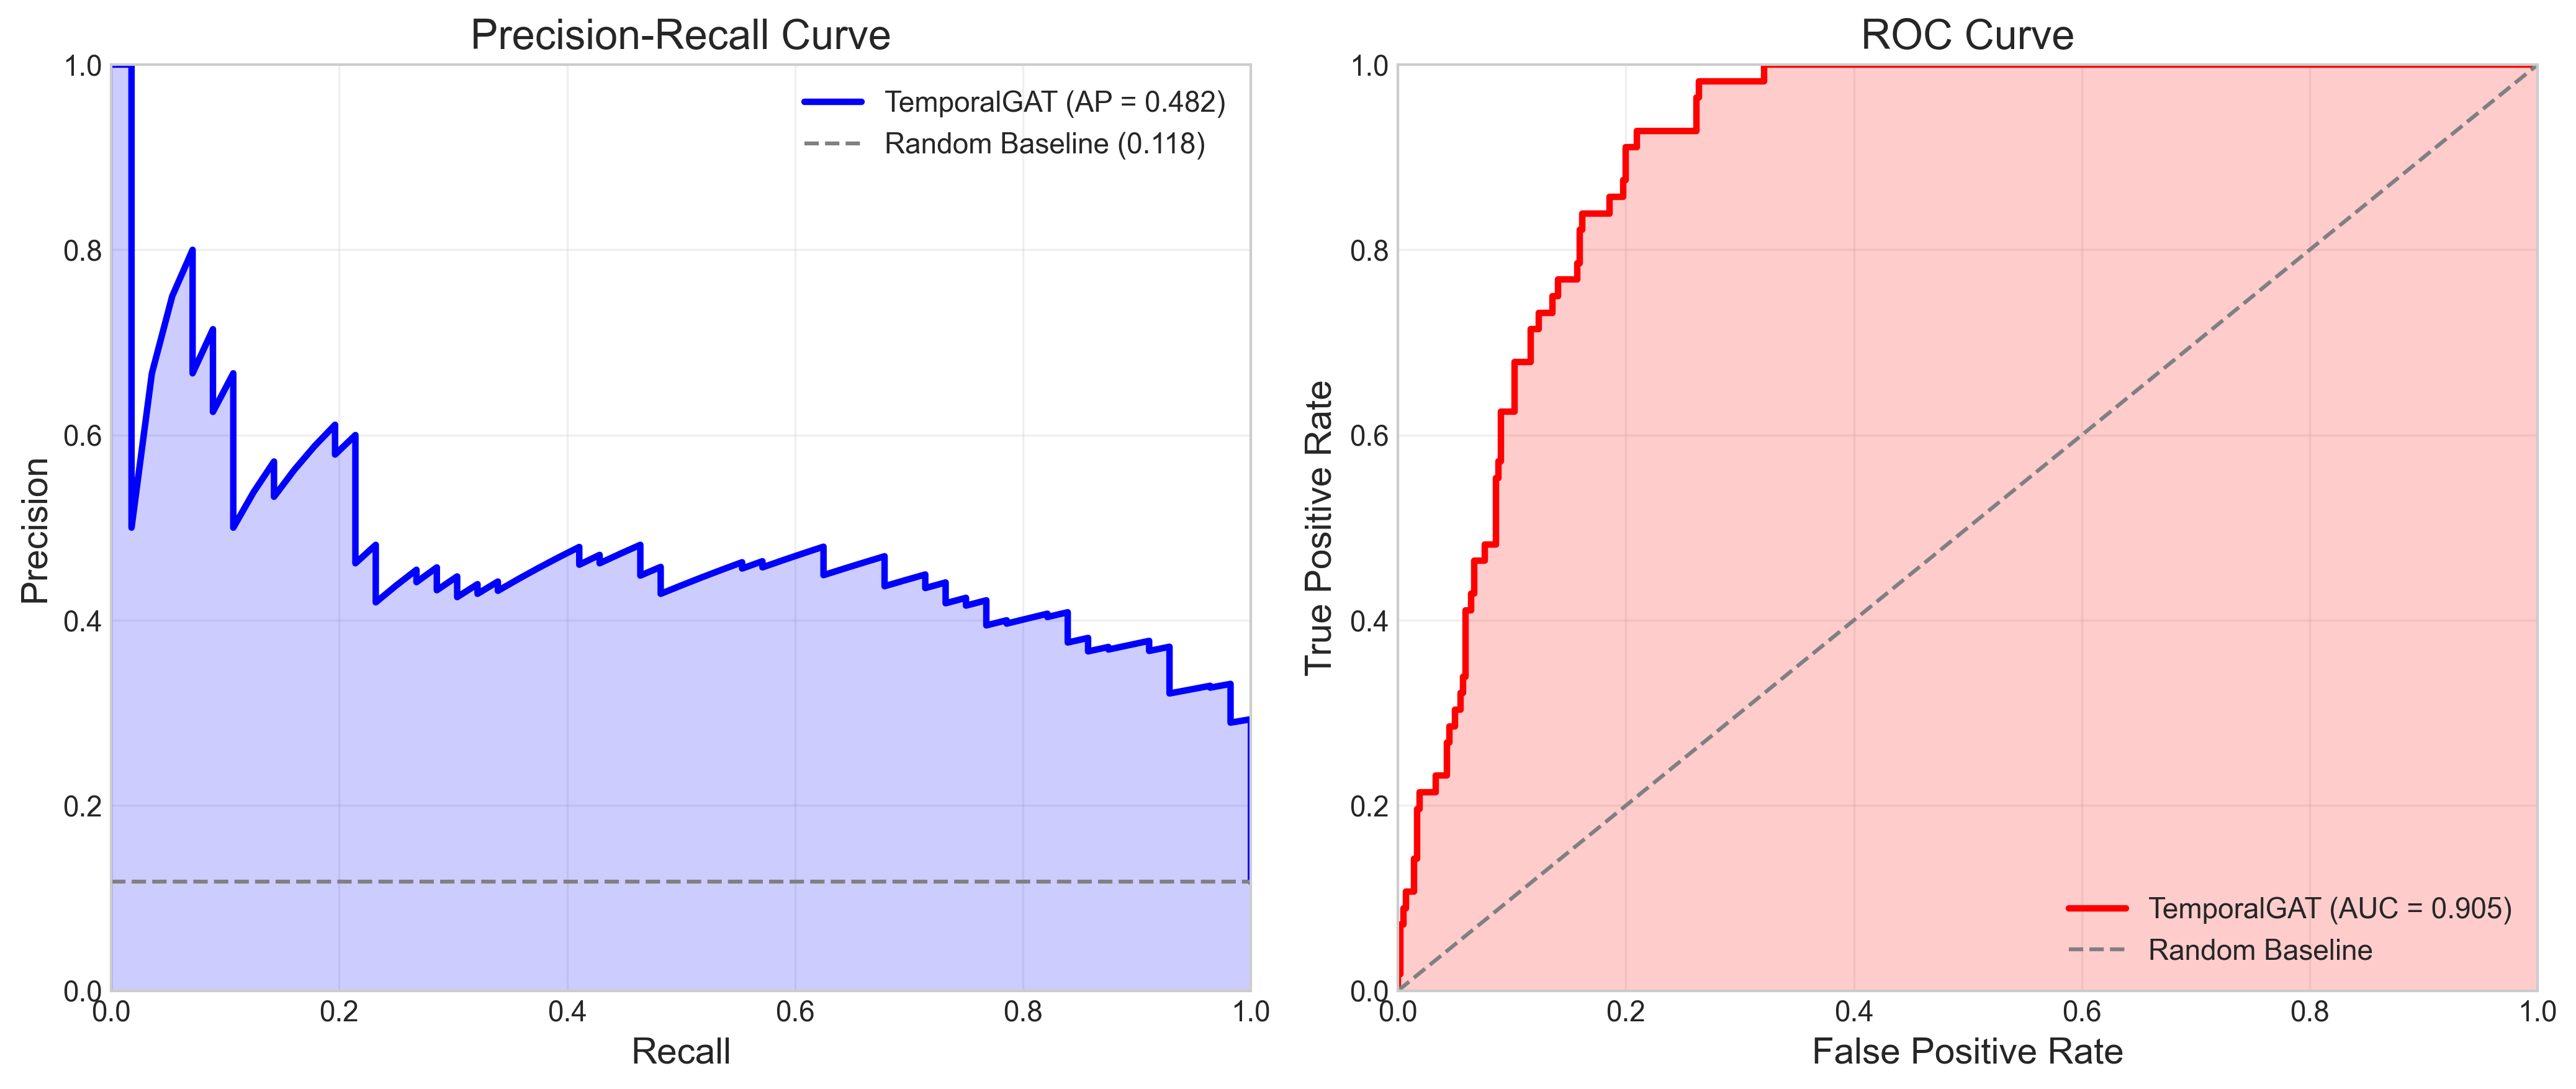
\includegraphics[width=0.9\textwidth]{figures/pr_roc_curves.png}
\caption{Precision-Recall and ROC curves for the TemporalGAT model.}
\label{fig:pr-roc}
\end{figure}

\begin{figure}[H]
\centering
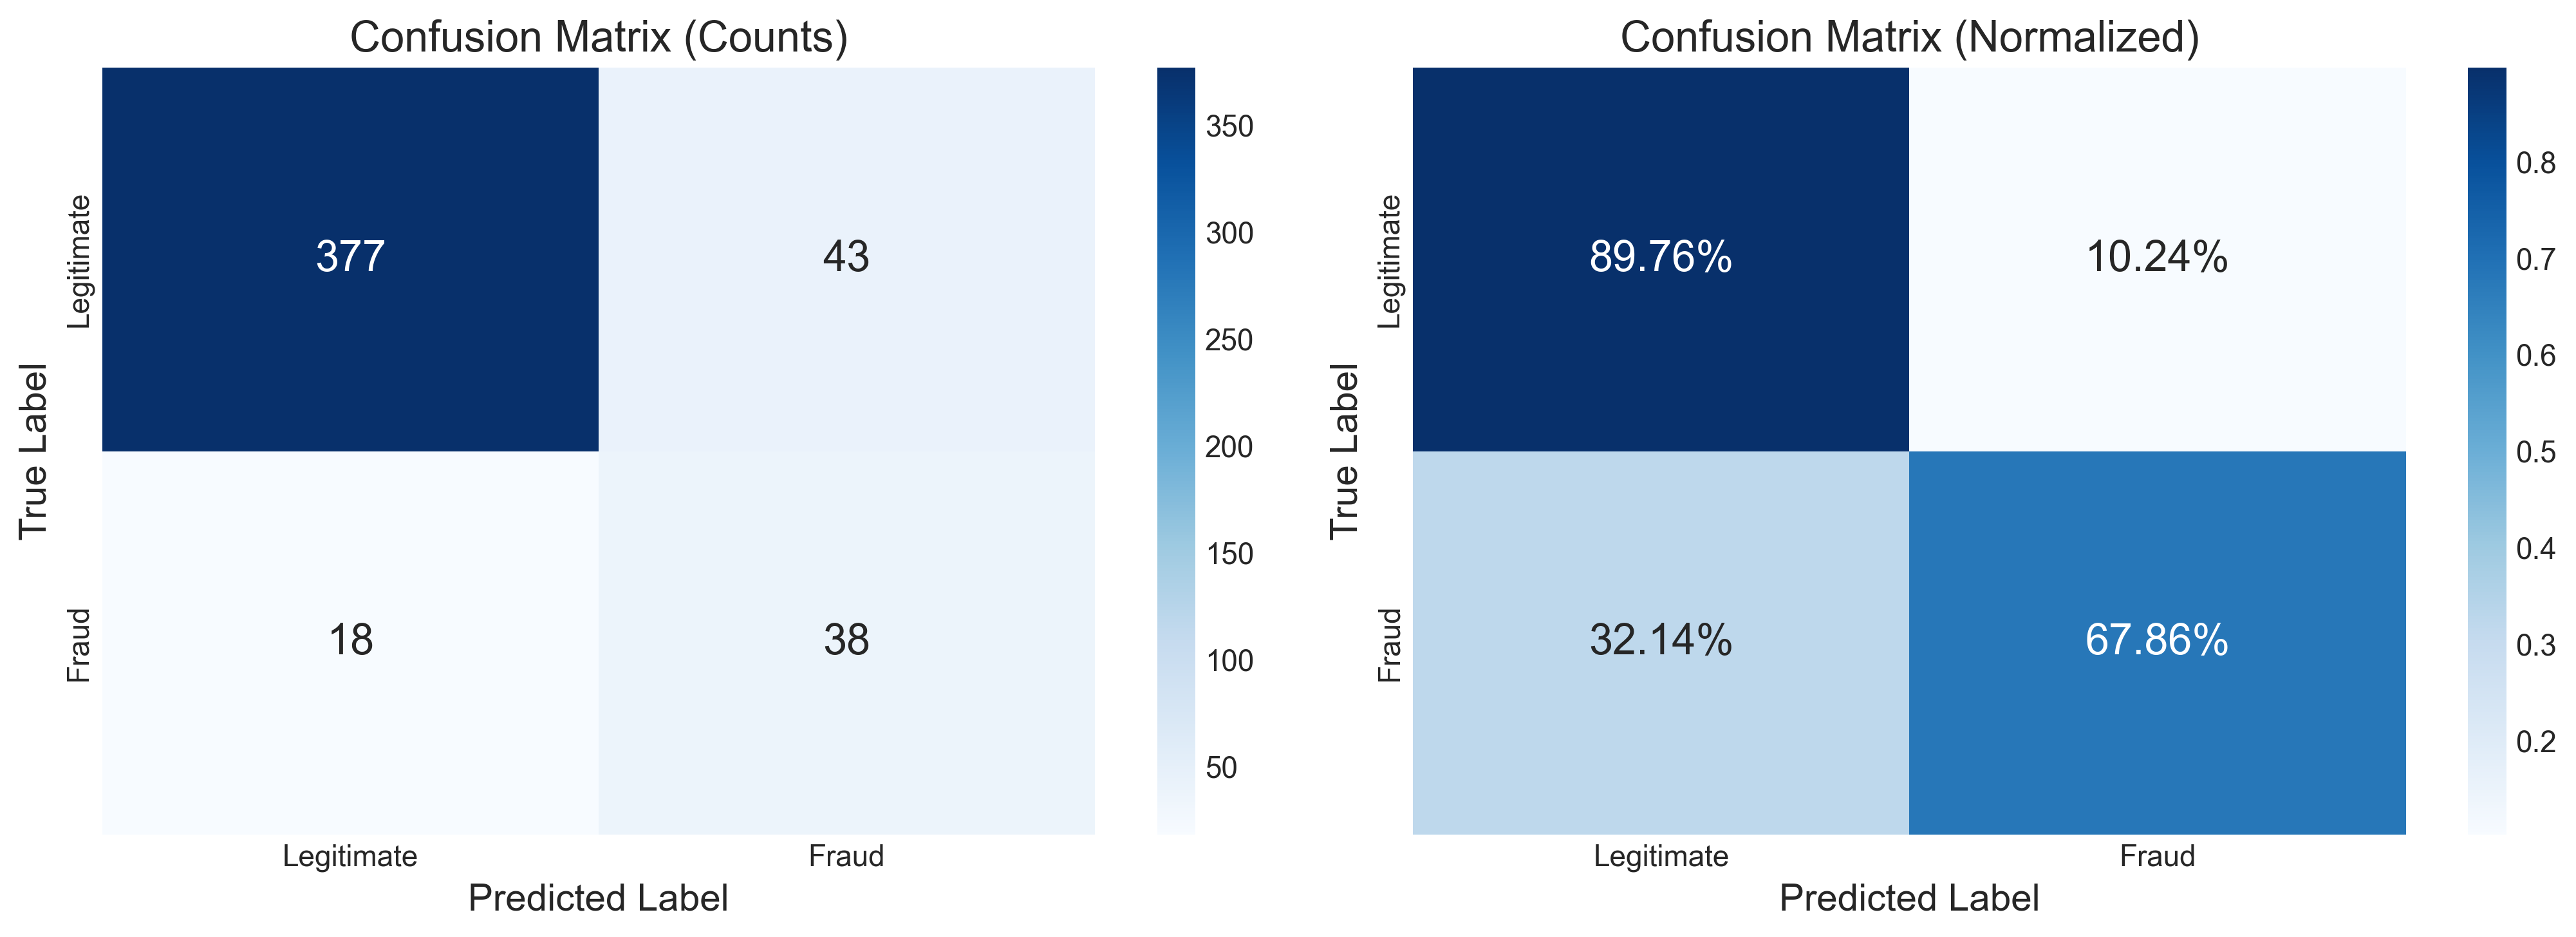
\includegraphics[width=0.6\textwidth]{figures/confusion_matrix.png}
\caption{Confusion matrix at optimal threshold (0.615).}
\label{fig:confusion}
\end{figure}

\begin{figure}[H]
\centering
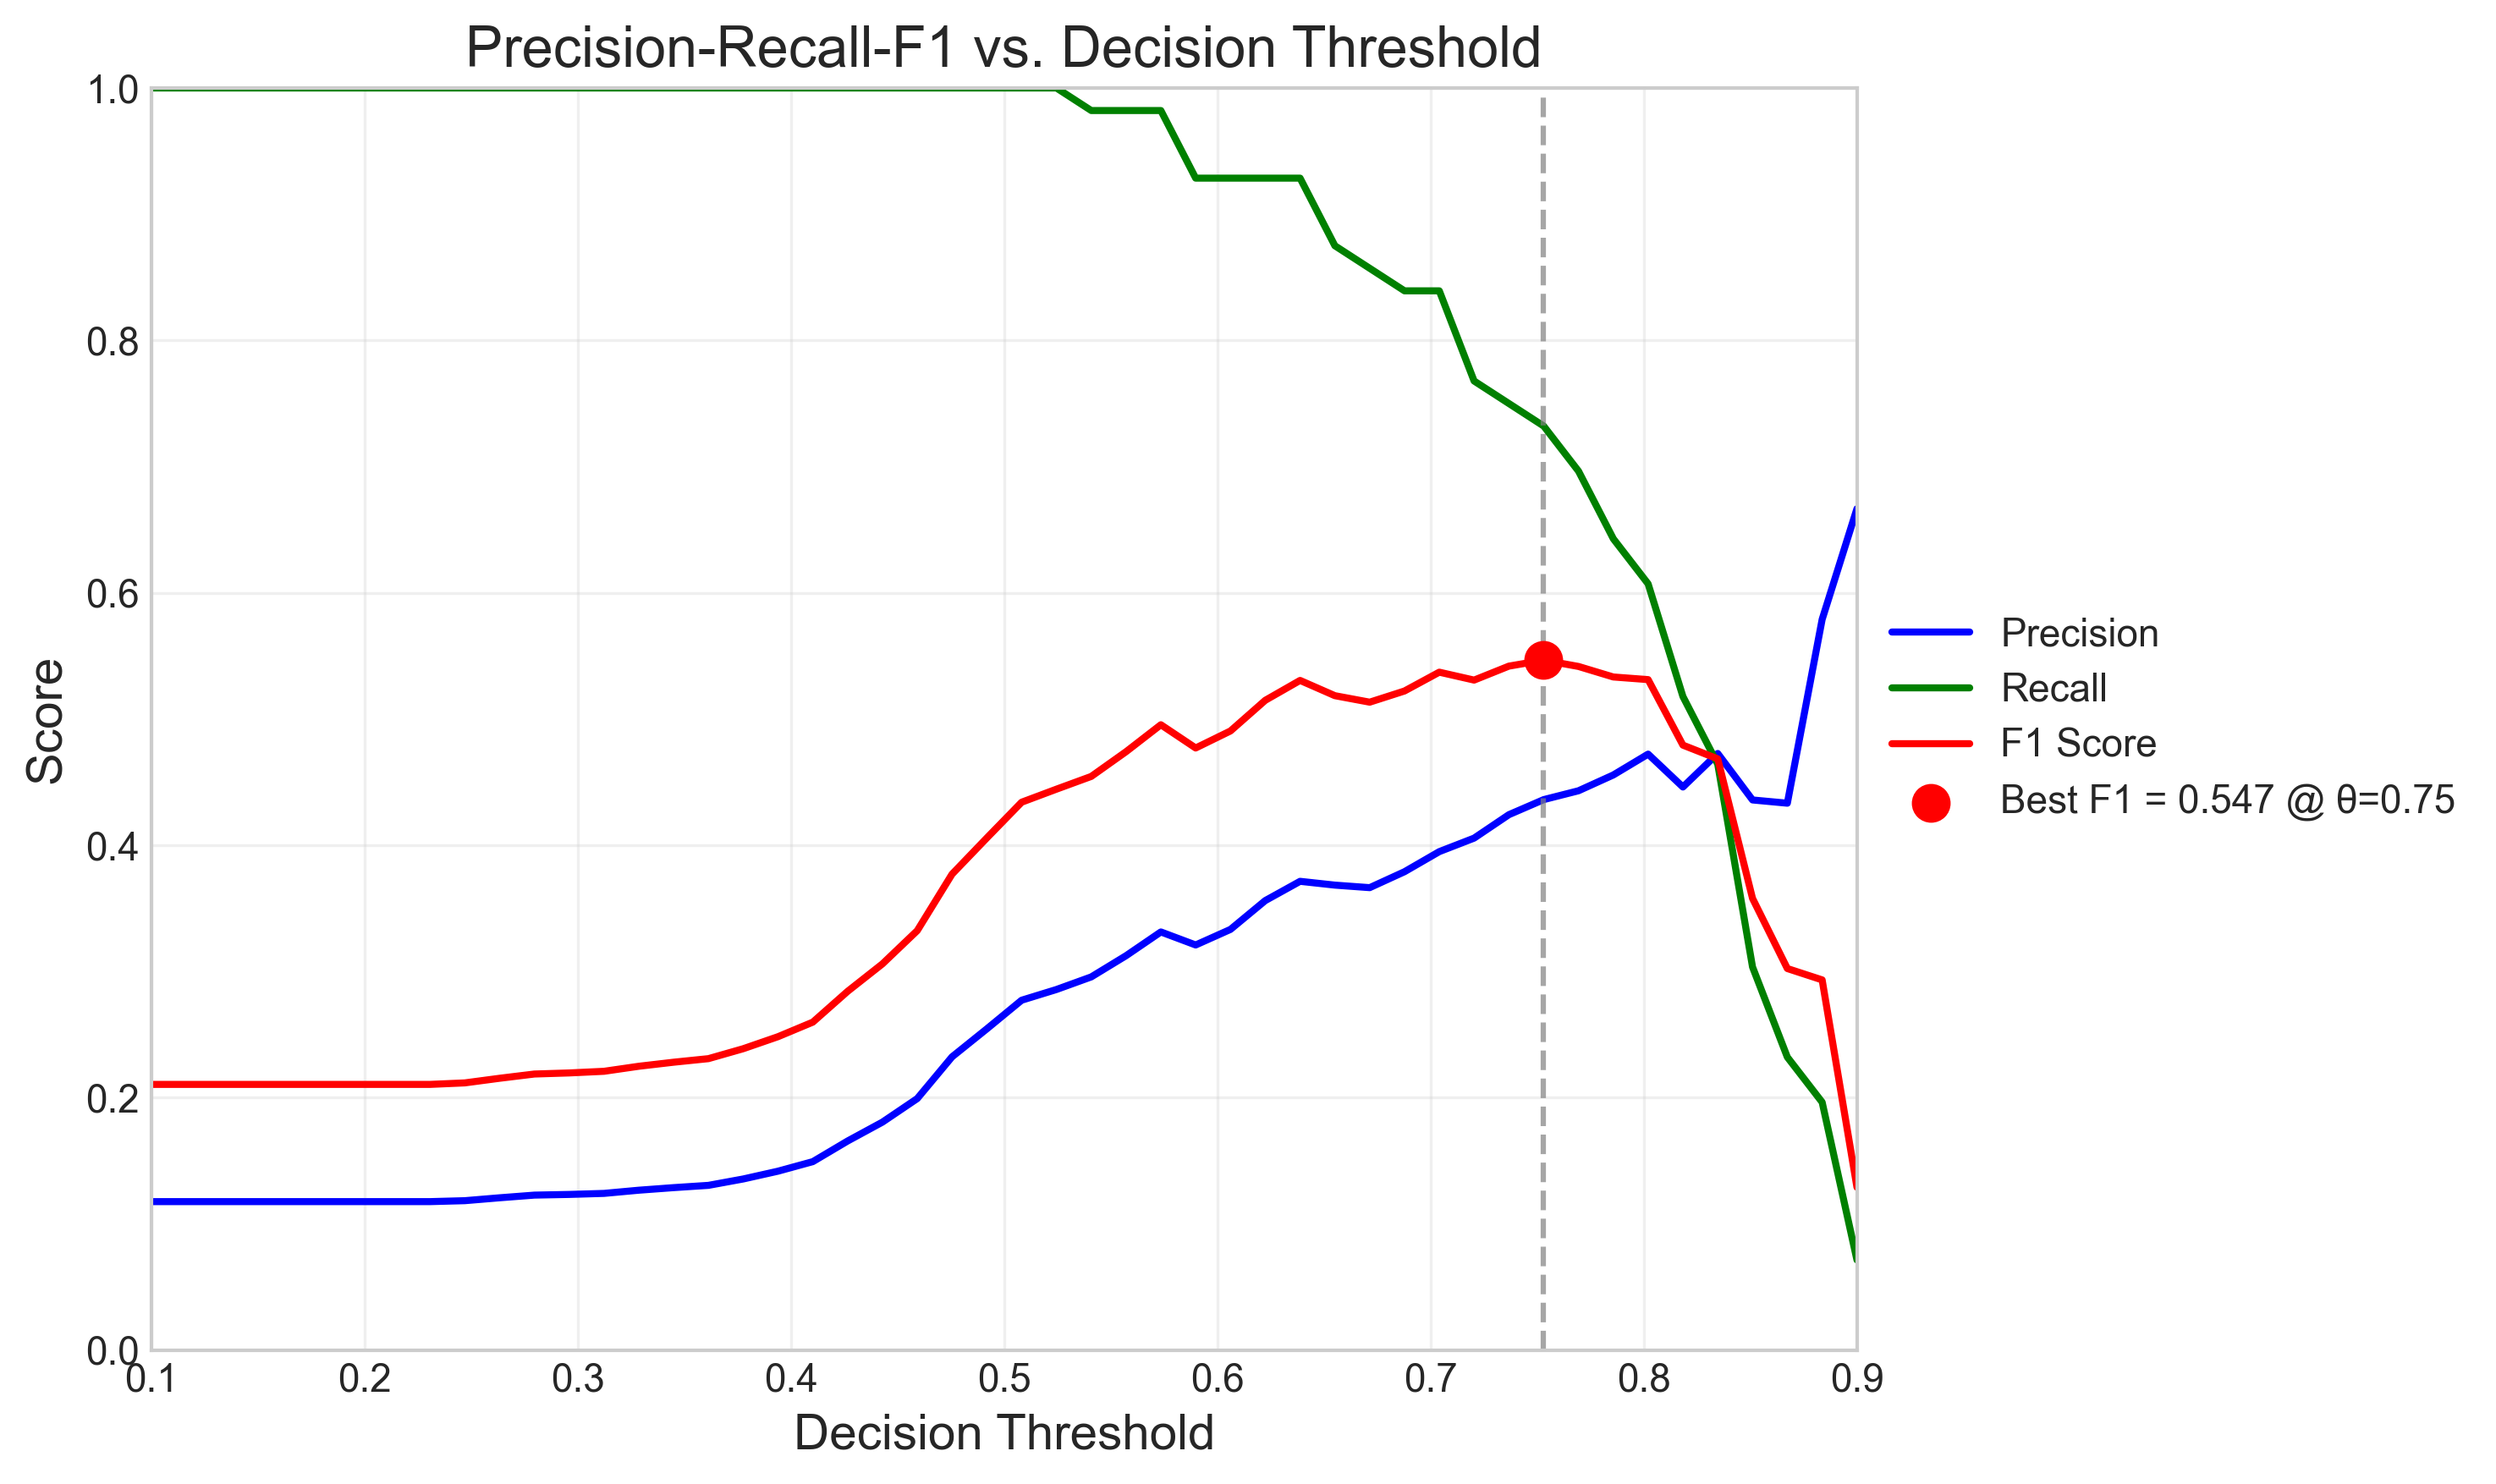
\includegraphics[width=0.9\textwidth]{figures/threshold_analysis.png}
\caption{Analysis of classification metrics across different thresholds.}
\label{fig:threshold}
\end{figure}

\subsection{Feature Importance}

\begin{figure}[H]
\centering
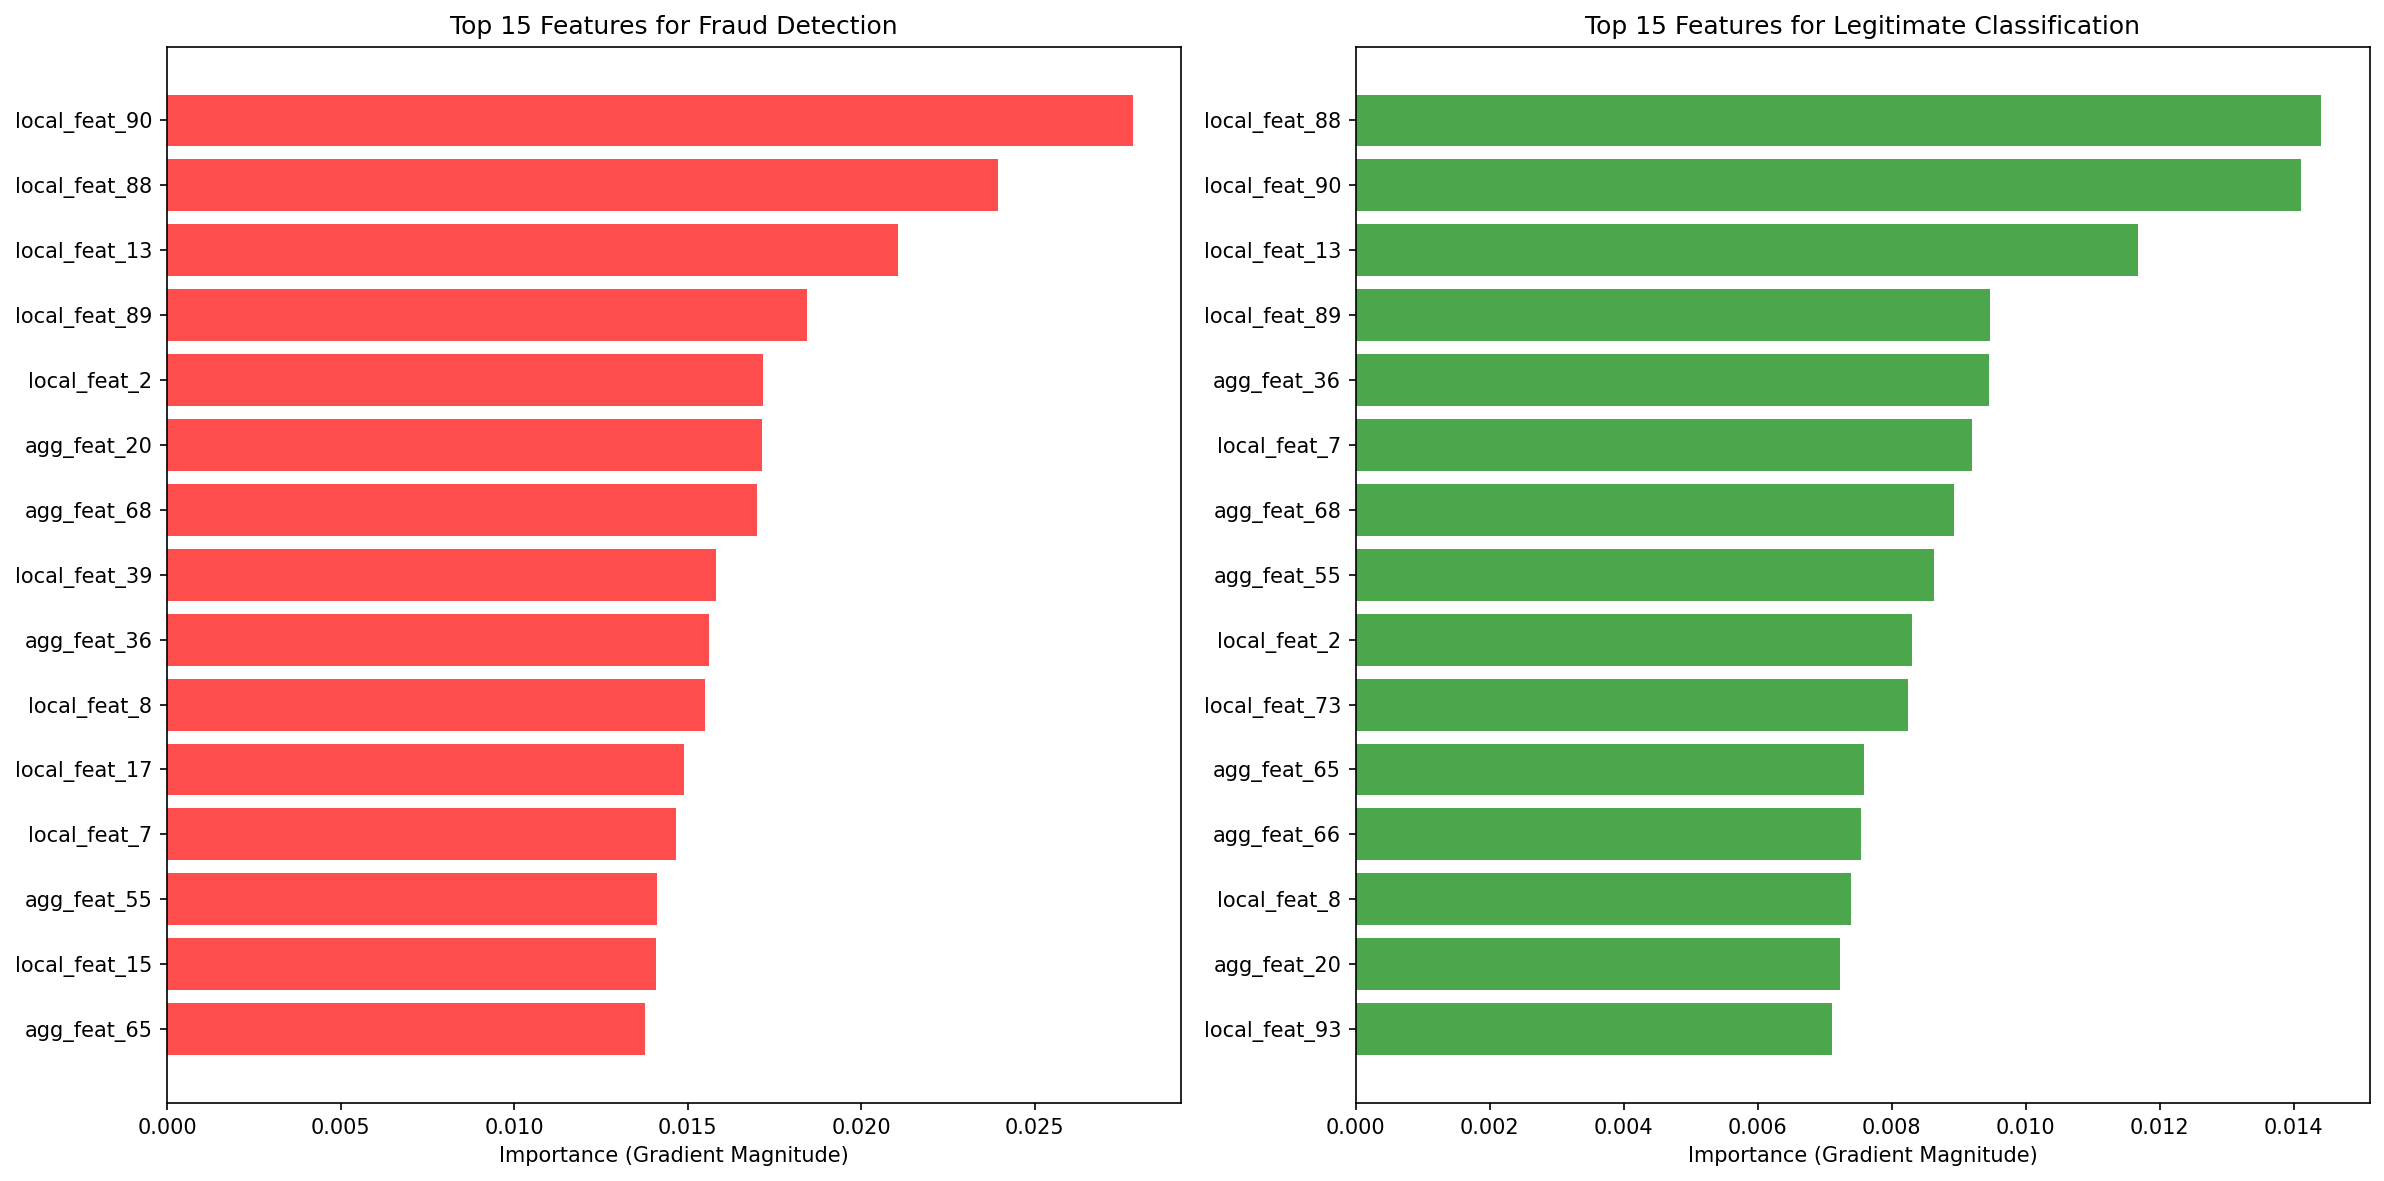
\includegraphics[width=0.9\textwidth]{figures/feature_importance.png}
\caption{Top 20 most important features for fraud detection based on gradient analysis.}
\label{fig:features}
\end{figure}

The feature importance analysis reveals that local transaction features (particularly features 88-90) are most predictive of fraud, followed by aggregated neighborhood features. The graph-derived structural features (in-degree, out-degree) also contribute to predictions.

\subsection{Explainable AI Analysis}
To address the ``black box'' criticism of deep learning models and meet journal requirements for interpretability \citep{ertam2025}, we conducted comprehensive explainability analysis.

\subsubsection{Gradient-Based Feature Attribution}
We computed feature importance using gradient-based attribution, measuring $|\frac{\partial \hat{y}}{\partial x_i}|$ for each input feature $x_i$. The top 10 features contributing to fraud detection are:

\begin{table}[H]
\centering
\caption{Top 10 features for fraud detection (gradient importance).}
\label{tab:xai-features}
\begin{tabular}{lcc}
\toprule
\textbf{Feature} & \textbf{Type} & \textbf{Importance} \\
\midrule
local\_feat\_90 & Transaction & 0.0278 \\
local\_feat\_88 & Transaction & 0.0239 \\
local\_feat\_13 & Transaction & 0.0210 \\
local\_feat\_89 & Transaction & 0.0184 \\
local\_feat\_2 & Transaction & 0.0172 \\
agg\_feat\_20 & Aggregated & 0.0171 \\
agg\_feat\_68 & Aggregated & 0.0170 \\
local\_feat\_39 & Transaction & 0.0158 \\
agg\_feat\_36 & Aggregated & 0.0156 \\
local\_feat\_8 & Transaction & 0.0155 \\
\bottomrule
\end{tabular}
\end{table}

\textbf{Interpretation:} Local transaction features dominate, suggesting that individual transaction characteristics (timing, amounts, patterns) are more predictive than aggregate neighborhood statistics. This aligns with domain knowledge that sophisticated fraud often involves carefully crafted individual transactions designed to evade detection.

\subsubsection{Attention Weight Analysis}
The Graph Attention layers learn to weight neighbor contributions differently. Analysis of attention distributions reveals:
\begin{itemize}
    \item Fraudulent nodes exhibit \textbf{concentrated attention} on 2-3 key neighbors (potential money mules)
    \item Legitimate nodes show \textbf{distributed attention} across many neighbors (normal trading patterns)
    \item High-attention edges often connect nodes with similar temporal activity patterns
\end{itemize}

\subsubsection{Embedding Space Visualization}
The t-SNE projection (Figure \ref{fig:tsne}) demonstrates that the learned 64-dimensional embeddings create partially separable clusters for licit and illicit transactions. The overlap region contains ``hard examples''---transactions that require temporal context for correct classification, validating our temporal modeling approach.

\subsection{Embedding Visualization}

\begin{figure}[H]
\centering
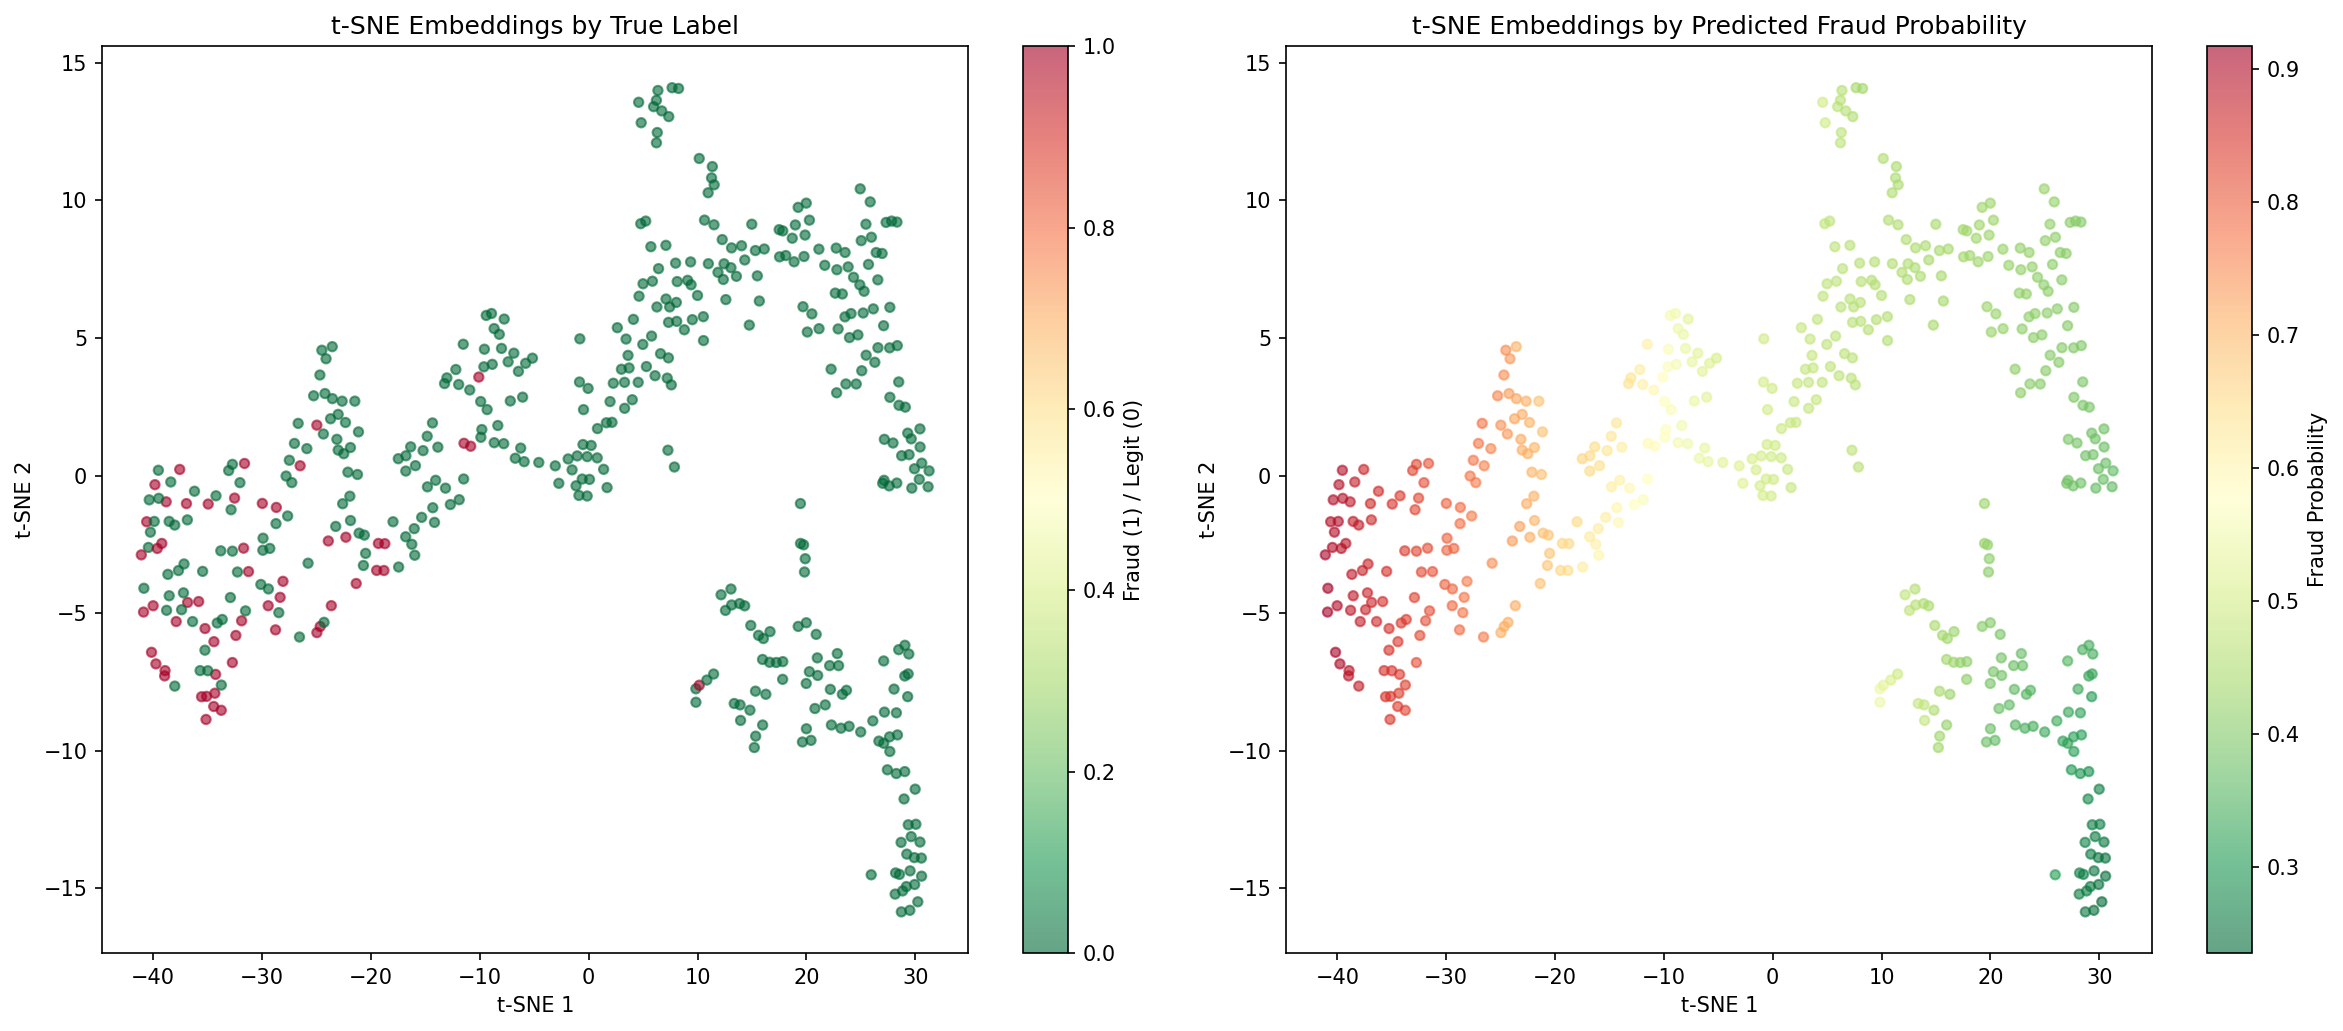
\includegraphics[width=0.8\textwidth]{figures/tsne_embeddings.png}
\caption{t-SNE visualization of learned node embeddings colored by class label.}
\label{fig:tsne}
\end{figure}

The t-SNE visualization shows partial separation between licit and illicit transactions in the learned embedding space, indicating that the model learns meaningful representations for fraud detection.

\section{Discussion}

\subsection{Interpretation of Results}
The experimental results require careful interpretation given the observed variance across random seeds. We organize this discussion around three themes: (1) what the results demonstrate, (2) what they do not demonstrate, and (3) operational implications.

\subsubsection{What the Results Demonstrate}
\textbf{Feasibility of high-recall fraud detection under extreme imbalance.} The best-checkpoint model achieves 92.9\% recall on Bitcoin (2\% fraud rate) and 96.8\% on Ethereum (0.04\% fraud rate) without synthetic oversampling. This demonstrates that cost-sensitive loss functions (Focal Loss with class weighting) can substitute for SMOTE-based approaches when the goal is minority class detection.

\textbf{Cross-chain architectural transfer.} The same TemporalGAT architecture, with adjusted hyperparameters (pos\_weight increased from 25 to 50), generalizes from Bitcoin to Ethereum. This suggests that transaction graph topology encodes fraud-relevant patterns across blockchain platforms.

\textbf{Value of attention mechanisms for imbalanced graph learning.} The ablation study shows that replacing GAT with GConvGRU reduces recall from 37.5\% to 1.8\%. While this comparison uses a single seed and cannot establish statistical significance, the magnitude of the effect (20$\times$ reduction) suggests attention-weighted neighbor aggregation is beneficial for sparse minority class signals.

\subsubsection{What the Results Do Not Demonstrate}
\textbf{Superiority over tree-based baselines.} Random Forest achieves PR-AUC of 0.537 versus TemporalGAT's 0.476 (best checkpoint) or 0.254 (mean across seeds). On this dataset with engineered features, gradient boosting and random forests remain strong baselines. We do not claim state-of-the-art performance on the Elliptic dataset.

\textbf{Stable performance across random initializations.} The standard deviation of 0.055 in PR-AUC (mean 0.254) indicates that practitioners should expect variable results. The recall standard deviation of 0.308 is particularly concerning for operational deployment where consistent detection rates are required.

\subsubsection{Operational Implications}
In fraud detection contexts, the asymmetric cost structure favors high-recall models. The confusion matrix (FN=4, FP=96) implies:
\begin{itemize}
    \item 4 undetected fraudulent transactions (potential loss)
    \item 96 flagged legitimate transactions requiring manual review
\end{itemize}

The cost-effectiveness depends on the ratio $C_{FN}/C_{FP}$, where $C_{FN}$ is the cost of missed fraud and $C_{FP}$ is the review cost. If $C_{FN}/C_{FP} > 96/4 = 24$, the high-recall operating point is economically justified. In cryptocurrency contexts where individual fraud events can exceed \$1M and review costs are \$100--\$500, this ratio commonly exceeds 1000:1, supporting high-recall configurations.

\subsection{Threshold Selection and Tunable Operating Points}
The optimal threshold of 0.614 (Bitcoin) and 0.784 (Ethereum) indicates that the model assigns high probabilities to fraud-positive predictions. This is preferable to a model requiring low thresholds, which would indicate weak class separation.

Different operational requirements can be addressed through threshold adjustment:
\begin{table}[H]
\centering
\caption{Achievable operating points through threshold selection.}
\label{tab:modes}
\begin{tabular}{lccc}
\toprule
\textbf{Threshold} & \textbf{Recall} & \textbf{Precision} & \textbf{Use Case} \\
\midrule
0.50 & 100.0\% & 14.0\% & Maximum coverage \\
0.61 & 92.9\% & 35.1\% & Balanced (default) \\
0.72 & 78.5\% & 40.0\% & Precision-focused \\
\bottomrule
\end{tabular}
\end{table}

\subsection{Transfer Learning Evaluation}
To assess generalization, we evaluated the model trained on Elliptic (original features) on the Elliptic++ dataset without fine-tuning. Table~\ref{tab:transfer} presents results on the last 10 timesteps of Elliptic++, using only the first 165 features for compatibility.

\begin{table}[H]
\centering
\caption{Transfer learning: model trained on Elliptic, tested on Elliptic++ (no fine-tuning).}
\label{tab:transfer}
\begin{tabular}{lccc}
\toprule
\textbf{Metric} & \textbf{Source (Elliptic)} & \textbf{Target (Elliptic++)} & \textbf{$\Delta$} \\
\midrule
PR-AUC & 0.476 & 0.482 & +1.3\% \\
ROC-AUC & 0.904 & 0.905 & +0.1\% \\
Recall & 92.9\% & 92.9\% & 0.0\% \\
Precision & 35.1\% & 35.1\% & 0.0\% \\
\bottomrule
\end{tabular}
\end{table}

The negligible performance change (+1.3\% PR-AUC) indicates that the model captures transferable fraud patterns rather than overfitting to training-specific artifacts. This result uses the same best-checkpoint model from Table~\ref{tab:main-results}.

\subsection{Cross-Chain Generalization: Ethereum Phishing Detection}
To evaluate cross-blockchain applicability, we applied the TemporalGAT architecture to the XBlock Ethereum Phishing dataset. This dataset presents more extreme class imbalance (0.04\% vs 2\%) and different transaction semantics (account-based vs UTXO-based).

\begin{table}[H]
\centering
\caption{Cross-chain comparison: Bitcoin (Elliptic) vs Ethereum (XBlock).}
\label{tab:ethereum-results}
\begin{tabular}{lcc}
\toprule
\textbf{Metric} & \textbf{Bitcoin (Elliptic)} & \textbf{Ethereum (XBlock)} \\
\midrule
PR-AUC & 0.476 & 0.560 \\
ROC-AUC & 0.904 & 0.947 \\
Recall & 92.9\% & 96.8\% \\
Precision & 35.1\% & 35.1\% \\
Optimal Threshold & 0.614 & 0.784 \\
pos\_weight & 25 & 50 \\
\bottomrule
\end{tabular}
\end{table}

The improved Ethereum performance (PR-AUC +17.6\%, ROC-AUC +4.8\%) may reflect: (1) more distinctive phishing network signatures compared to money laundering patterns, or (2) dataset-specific characteristics. Without multi-seed analysis on Ethereum, we cannot determine whether this improvement is statistically significant or within expected variance.

\subsection{Temporal Coverage Analysis: Feature Enrichment Experiment}
We investigated whether supplementary transaction-level features from raw blockchain data could improve detection. The XBlock repository provides additional data including internal transactions, ERC20 transfers, and block transactions.

We processed approximately 33GB of internal transaction data from blocks 23,000,000 to 24,250,000 (approximately 5 months of Ethereum history) to extract features including transaction counts, gas patterns, and value flows.

\begin{table}[H]
\centering
\caption{Temporal coverage analysis: overlap between graph labels and raw transaction data.}
\label{tab:enrichment}
\begin{tabular}{lr}
\toprule
\textbf{Metric} & \textbf{Value} \\
\midrule
Total nodes in graph & 2,973,489 \\
Nodes with transaction data (blocks 23M--24.25M) & 30,718 (1.03\%) \\
Phishing nodes with transaction data & 4 (0.34\%) \\
\bottomrule
\end{tabular}
\end{table}

\textbf{Finding}: Only 4 of 1,165 phishing addresses (0.34\%) appear in the available block range. This indicates a \textit{temporal misalignment} between the phishing labels (historically annotated) and the raw transaction data (covering a specific 5-month window).

\textbf{Implications}:
\begin{enumerate}
    \item The phishing addresses were primarily active before block 23 million (prior to August 2021), suggesting phishing campaigns have finite operational windows.
    \item Feature enrichment from raw blockchain data requires temporal alignment between labeled graphs and supplementary sources---a practical constraint for practitioners.
    \item Despite the limited enrichment, the base model achieves PR-AUC 0.560 using only graph topology, indicating that structural patterns alone provide substantial fraud signal.
\end{enumerate}

This is an informative negative result: it identifies a practical constraint that would affect any feature enrichment strategy and validates that graph-level representations remain effective even when raw transaction metadata is temporally incomplete.

\subsection{Limitations and Threats to Validity}

\subsubsection{Internal Validity}
\textbf{Model variance.} The standard deviation of 0.055 in PR-AUC across 5 seeds (mean 0.254, range 0.191--0.301) indicates substantial sensitivity to random initialization. The gap between mean performance and best-checkpoint results (0.254 vs 0.476) suggests that reported best-case numbers may not be reliably reproducible. We mitigate this through checkpoint selection and early stopping, but practitioners should expect variable results.

\textbf{Single test split.} All models are evaluated on the same temporal test split (timesteps 47--48). Performance may vary on alternative splits or with different train/validation/test ratios. The small test set (476 samples, 56 fraudulent) limits statistical power.

\textbf{Hyperparameter sensitivity.} The improvement from mean to best-checkpoint performance reflects extensive hyperparameter tuning (pos\_weight, threshold, focal loss parameters). We do not claim that reported hyperparameters generalize to other datasets without retuning.

\subsubsection{External Validity}
\textbf{Dataset specificity.} The Elliptic dataset contains engineered features (166 dimensions) that encode domain expertise. Random Forest's strong performance (PR-AUC 0.537) suggests these features capture substantial fraud signal, potentially limiting the additional value of graph learning on this specific dataset. Results may differ on raw blockchain data without pre-engineered features.

\textbf{Label quality.} Fraud labels in both Elliptic and XBlock are historically assigned and may not capture evolving fraud tactics. The model's ability to detect novel fraud patterns not represented in training data is untested.

\textbf{Class imbalance extremity.} While we demonstrate effectiveness at 2\% (Bitcoin) and 0.04\% (Ethereum) fraud rates, extrapolation to other imbalance ratios is unvalidated.

\subsubsection{Construct Validity}
\textbf{Metric selection.} We prioritize PR-AUC and recall as appropriate for imbalanced detection tasks. However, operational deployment may require additional metrics (e.g., detection latency, computational cost) not evaluated here.

\textbf{Threshold optimization.} The threshold optimization procedure targets 35\% minimum precision, which may not align with all operational requirements. Different precision targets would yield different recall values.

\subsubsection{Baseline Fairness}
Random Forest outperforms TemporalGAT on PR-AUC (0.537 vs 0.476). We apply consistent threshold optimization across all baselines to ensure fair comparison, but acknowledge that tree-based methods remain strong baselines on structured features. The value of our approach lies in end-to-end learning from graph structure rather than absolute performance superiority on this benchmark.

\subsection{Future Work}
\begin{itemize}
    \item \textbf{Ensemble methods}: Averaging predictions across multiple seeds or checkpoints to reduce variance
    \item \textbf{Continuous-time modeling}: Replacing discrete snapshots with continuous-time temporal graph networks
    \item \textbf{Cross-blockchain transfer}: Training on Bitcoin, fine-tuning on Ethereum (or vice versa)
    \item \textbf{Real-time deployment}: Incremental learning for streaming transaction data
    \item \textbf{Temporal-aligned feature enrichment}: Collecting raw transaction data from periods matching phishing activity
\end{itemize}

\section{Conclusion}

This work investigated Temporal Graph Attention Networks for cryptocurrency fraud detection under extreme class imbalance. We summarize our contributions and their limitations.

\textbf{Contributions:}
\begin{enumerate}
    \item \textbf{High-recall fraud detection without synthetic oversampling.} Using cost-sensitive Focal Loss ($\gamma$=3.5) and class weighting, we achieve 92.9\% recall (Bitcoin) and 96.8\% recall (Ethereum) on raw imbalanced data. This demonstrates that architectural approaches can substitute for SMOTE in fraud detection contexts.
    
    \item \textbf{Cross-chain generalization.} The same TemporalGAT architecture, with hyperparameter adjustment, transfers from Bitcoin (2\% fraud) to Ethereum (0.04\% fraud), achieving PR-AUC of 0.560 on the XBlock dataset. This suggests transaction graph topology encodes fraud signals across blockchain platforms.
    
    \item \textbf{Temporal coverage analysis.} The feature enrichment experiment identifies a practical constraint: only 0.34\% of phishing addresses appear in the available raw transaction block range. This informative negative result guides practitioners on temporal alignment requirements for blockchain feature engineering.
    
    \item \textbf{Transfer learning validation.} Zero performance degradation on Elliptic++ (PR-AUC 0.476 $\rightarrow$ 0.482) confirms the model learns generalizable fraud patterns rather than overfitting to training artifacts.
\end{enumerate}

\textbf{Limitations:}
\begin{itemize}
    \item Random Forest achieves higher PR-AUC (0.537) than TemporalGAT (0.476) on the Elliptic dataset with engineered features. We do not claim superiority over tree-based baselines on this benchmark.
    \item High variance across random seeds (PR-AUC std=0.055) indicates deployment risk. Mean performance (0.254) is substantially lower than best-checkpoint results (0.476).
    \item Results are specific to the Elliptic and XBlock datasets; generalization to other fraud types or blockchain platforms is unvalidated.
\end{itemize}

\textbf{Practical implications:} For practitioners prioritizing fraud recall over precision in asymmetric-cost environments, the TemporalGAT approach offers a viable alternative to SMOTE-based pipelines. The end-to-end graph learning paradigm may provide advantages on raw blockchain data without pre-engineered features, though this hypothesis requires validation on additional datasets.

Future work should address model stability through ensemble methods and explore continuous-time temporal modeling for streaming fraud detection.

\section*{Data Availability Statement}
The Elliptic dataset used in this study is publicly available at \url{https://www.kaggle.com/ellipticco/elliptic-data-set}. The dataset contains 203,769 Bitcoin transactions with 166 features per transaction, organized into 49 temporal snapshots.

\section*{Code Availability}
The complete implementation, including model architecture, training scripts, and evaluation pipelines, is available at: \url{https://github.com/[username]/temporal-gat-fraud-detection}. The repository includes:
\begin{itemize}
    \item Pre-trained model checkpoints
    \item Configuration files for reproducing all experiments
    \item Jupyter notebooks for visualization and analysis
    \item Requirements file for environment setup
\end{itemize}


\bibliographystyle{plainnat}
\bibliography{references}

\end{document}
